\documentclass[titlepage]{article}
\title{Tietokantojen perusteiden ryhm\"aty\"o - keskustelupalsta}
\author{Valtteri Eskola 014471751, \\ Anne Kiirikki 014420773, \\ Joel Petro 014428047, \\ Vesa Riekkinen 013613345}
\date{}

\usepackage[utf8]{inputenc}
\usepackage[T1]{fontenc}
\usepackage[finnish]{babel}
\usepackage{graphicx}
\usepackage{float}
\usepackage{hyperref} 

\begin{document}
\maketitle

\noindent Web-sovelluksen osoite: % \href{Tähän osoite}{tähän osoite} \\
Web-sovelluksen koodit: \href{https://github.com/vesarie/palsta}{https://github.com/vesarie/palsta} \\

\section*{Käsitekaavio}
Tarpeelliset käsitteet ovat alue, keskustelu ja viesti. Kuvassa \ref{käsite} näkyvät niiden väliset osallitumisrajoitteet ja riippuvuudet.

\begin{figure}[H]
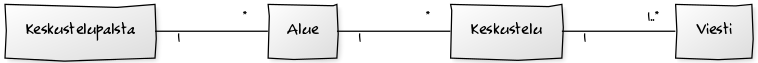
\includegraphics[width=\textwidth]{kasitekaavio}
\label{käsite}
\caption{Keskustelupalstan osallistumisrajoitteet}
\end{figure}

\section*{Attribuutit}

\noindent Taulukossa on listattu kunkin taulun tarvitsemat attribuutit ja avaimet. \\

{
\centering
\begin{tabular}[width=\textwidth]{r|l}

Käsite & Attribuutit \\
\hline
Alue & (pk) tunnus integer, nimi varchar(), web{\_}tunnus varchar(n) \\
Keskustelu & (pk) tunnus integer , (fk) alue : Alue,  otsikko varchar(n), \\ 
		& web{\_}tunnus varchar(n) \\
Viesti & (pk) tunnus, (fk) keskustelu : Keskustelu, pvm TIMESTAMP, \\ 
		& sisalto varchar(n), web{\_}tunnus varchar(n) \\
\end{tabular}
} \\

\section*{Tietokantakaavio}

\begin{figure}[H]
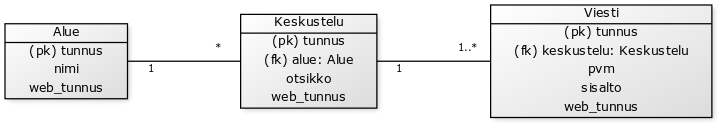
\includegraphics[width=\textwidth]{tietokantakaavio}
\label{tkkaavio}
\caption{Tietokantakaavio}
\end{figure}

\section*{Taulujen luonti SQL-komennoilla}

CREATE TABLE Alue ( 
\begin{itemize}
	\item[] tunnus integer PRIMARY KEY,
    \item[] web{\_}tunnus varchar(100) NOT NULL UNIQUE,
    \item[] nimi varchar(100) NOT NULL,
\end{itemize}
); \\

CREATE TABLE Keskustelu ( 
\begin{itemize}
	\item[] tunnus integer PRIMARY KEY,
    \item[] alue integer NOT NULL,
    \item[] web{\_}tunnus integer NOT NULL UNIQUE,
    \item[] otsikko varchar(250) NOT NULL,
    \item[] FOREIGN KEY(alue) REFERENCES Alue(tunnus)

\end{itemize}
); \\

CREATE TABLE Viesti ( 
\begin{itemize}
	\item[] tunnus integer PRIMARY KEY,
    \item[] keskustelu integer NOT NULL,
    \item[] lahettaja varchar(100) NOT NULL,
    \item[] pvm TIMESTAMP NOT NULL,
    \item[] web{\_}tunnus integer NOT NULL,
    \item[] sisalto text NOT NULL,
    \item[] FOREIGN KEY(keskustelu) REFERENCES Keskustelu(tunnus)


\end{itemize}
); \\

\section*{Muutamia keskeisiä käyttötapauksia}

Joitain keskeisiä käyttötapauksia ovat

\subsection*{Alueiden listaus}

SELECT a.nimi AS alue, COUNT(v.tunnus) AS viesteja, \\ MAX(v.pvm) AS viimeisin 
FROM Alue a
\begin{itemize}
	\item[] LEFT JOIN Keskustelu k ON a.tunnus = k.alue
    \item[] INNER JOIN Viesti v ON k.tunnus = v.keskustelu
\end{itemize}
GROUP BY a.tunnus
ORDER BY alue

Komennossa haetaan kaikki alueet, niiden sisältämien viestien lukumäärä ja uusimman viestin lähetysaika. Listaus on ryhmitelty alueen tunnuksen perusteella ja aakkosjärjestyksessä alueen nimen mukaan. 

\subsection*{Alueen sisältämien keskustelujen listaaminen}

SELECT k.otsikko AS keskustelu, COUNT(v.tunnus) AS viesteja, \\ MAX(v.pvm) AS viimeisin 
FROM Alue a
\begin{itemize}
  \item[] INNER JOIN Keskustelu k ON a.tunnus = k.alue
  \item[] LEFT JOIN Viesti v ON k.tunnus = v.keskustelu
\end{itemize}
WHERE alue.web{\_}tunnus = ? \\
GROUP BY k.tunnus \\
ORDER BY viimeisin DESC \\
LIMIT 10 OFFSET ? \\

Kysely listaa kymmenen tuoreinta keskustelua viimeisimmän viestin perusteella ja kunkin keskustelun viestien lukumäärän. 


\subsection*{Viestin lisääminen}

INSERT INTO Viesti (keskustelu, sisalto) VALUES (?,?); \\

\noindent Kysymysmerkit viittaavat keskusteluun ja sisältöön.

\section*{Ongelmia}

Ei ole vielä


\section*{Jatkokehitysmahdollisuuksia}

Keskutelupalstaa voisi hienosäätää esimerkiksi siten, että käyttäjä voisi kirjautua sisään tunnuksella ja salasanalla. Viestien lisäystä voisi monipuolistaa luomalla mahdollisuuden lisätä linkkejä, kuvia ja lainata toisten käyttäjien viestejä. Keskustelupalstalle voisi lisätä hakuominaisuuden ja pakollisen "Jaa Facebookissa" -napin. Sivuston ulkoasu voisi olla kauniimpi. Navigointipalkki voisi helpottaa sivustolla liikkumista. Keskustelut, joihin on tullut uusia viestejä, voisivat näkyä korostetusti käyttäjälle. Nettirikollisuuden kitkemiseksi tarvitaan Nettivinkki-pikalinkki 

\end{document}
